\section{Problema aziendale}
\subsection{Descrizione generale}
L'azienda AP srl di Reggio Emilia è un'\textbf{azienda manifatturiera} specializzata nel settore metallurgico. \\
L'impresa si occupa di lavorazione, trattamento e rifinitura di metalli semilavorati in metallo e leghe per conto terzi. \\
L'azienda vuole migliorare l'efficenza dei suoi \textbf{processi produttivi} per riuscire ad essere più competitiva nel mercato.
I loro processi partono da un prodotto grezzo che deve essere lavorato da una delle macchine presenti in azienda.\\
L'azienda ha un magazzino interno per ospitare prodotti grezzi e prodotti finiti, in questo studio non viene considerata una capienza massima.\\
Nel problema viene considerato un periodo di N giorni, dove i prodotti grezzi sono già presenti in magazzino, e al termine del periodo bisogna soddisfare scadenze dei cliente con le quantità di prodotto finito desiderate.\\
\paragraph*{Obiettivo} L'azienda vuole una \textbf{schedulazione} di N giorni dove vengono indicate le lavorazioni da assegnare alle macchine e il numero di prodotti da ottenere. \\
La schedulazione deve rispettare i vincoli del problema e soprattuto raggiungere le quantità richieste dai clienti.\\
La soluzione deve ridurre i costi legati al cambio configurazione e all'utilizzo superfluo di macchine, cercando di ottenere idealmente solo macchine che lavorano.
\subsection{Analisi processo produttivo}
Il processo è formato da \textbf{diverse fasi} (come si può notare anche in figura \ref{fig:fasi_di_produzione}):
\begin{enumerate}
    \item Configurazione macchina (tempo constante).
    \item L'operatore posiziona il prodotto grezzo in uno dei pallet dedicato della macchina. (tempo constante)
    \item La macchina effettua la lavorazione. (tempo dinamico, dipende dal prodotto)
    \item L'operatore controlla il prodotto lavorato, effettua i vari test qualità e sposta il prodotto finito fuori dalla macchina (tempo constante).
    \item Pulizia macchina (tempo constante).
\end{enumerate}
\begin{figure}[H]
    \centering
    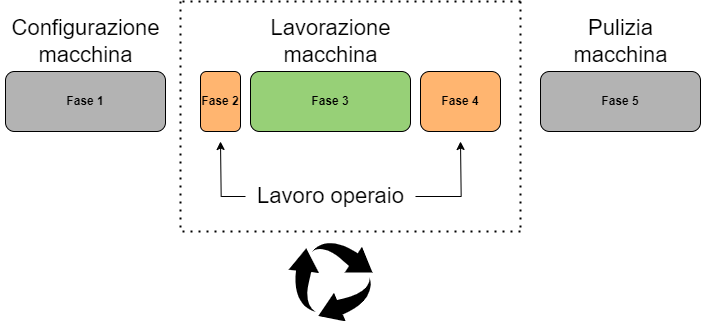
\includegraphics[width=\textwidth]{media/fasi_di_produzione.drawio.png}
    \caption{Fasi di produzione}
    \label{fig:fasi_di_produzione}
\end{figure}
Per ottenere un prodotto è necessario disporre il prodotto grezzo, aspettare la lavorazione della macchina e controllare il prodotto finito.\\
La prima e l'ultima fase sono presenti una sola volta agli estremi dell'intero processo produttivo, mentre le fasi 2, 3 e 4 vengono ripetute ciclicamente per raggiungere la quantità di prodotto desiderata.\\ 
Quindi per produrre 100 prodotti, sarà necessario configurare la macchina, effettuare 100 cicli di lavorazione e pulire la macchina.
\\ \\
In questo modo si può creare una pipeline di produzione come si può notare in figura \ref{fig:pipeline_di_produzione}, e parallelizzare il lavoro della macchina con quello dell'operatore.
\begin{figure}[H]
    \centering
    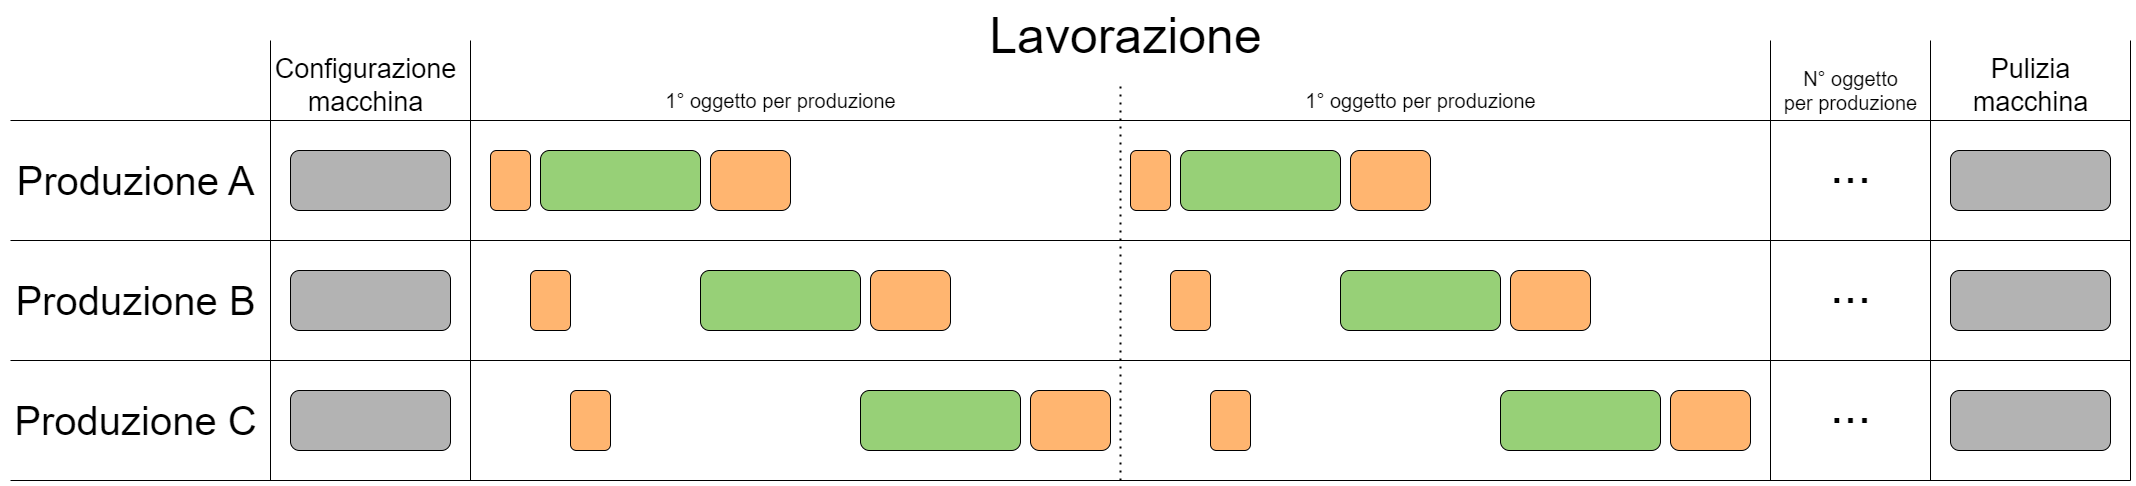
\includegraphics[width=\textwidth]{media/pipeline.drawio.png}
    \caption{Pipeline di produzione su una macchina}
    \label{fig:pipeline_di_produzione}
\end{figure}
L'operatore posiziona il primo pezzo, fa partire la lavorazione e nel mentre posiziona l'altro pezzo da lavorare. \\
Allo stesso modo l'operatore può controllare il prodotto finito nel mentre che la macchina lavora su un altro pezzo.\\
Analizzando un ciclo della lavorazione in pipeline (in figura \ref{fig:analisi_ciclo_di_produzione}), il tempo di lavorazione dell'operaio si paga \textbf{per un solo prodotto} rispetto agli N prodotti: fase 2 primo prodotto e fase 4 ultimo prodotto;\\
mentre il restante tempo necessario alla lavorazione dell'operaio è coperto dalla lavorazione della macchina.
Questo porta ad un risparmio di tempo, ma si ha un ciclo di produzione più lungo: ottenere 1 prodotto finito di ogni N prodotti, è necessario aspettare la lavorazione di tutti gli N prodotti.
\begin{figure}[H]
    \centering
    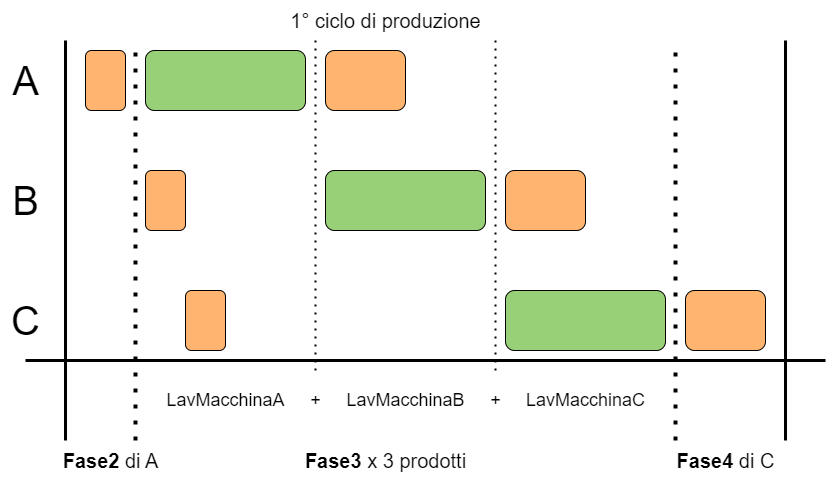
\includegraphics[width=\textwidth]{media/analisi_ciclo.drawio.png}
    \caption{Analisi singolo ciclo di produzione}
    \label{fig:analisi_ciclo_di_produzione}
\end{figure}
I tempi delle diverse fasi di produzioni possono essere semplificate come segue:
\begin{enumerate}
    \item \(TIME\_MACHINE\_SETUP\) : tempo configurazione e pulizia macchina (fase 1 e fase 5).
    \item \(TIME\_OPERATOR\) : tempo di lavorazione manuale (fase 2 e fase 4).
    \item \(time\_machine_w\) : tempo di lavorazione automatica della macchina (fase 3).
\end{enumerate}
I primi due sono tempi costanti, mentre il tempo di lavorazione della macchina dipende dal prodotto da lavorare.\\
L'algoritmo dovrà scegliere quanti e quali lavorazioni fare in una determinata macchina e quale quantità di prodotto raggiungere.\\
Queste scelte vengono definite come \textbf{Jobs} e sono formati da una lista di lavorazioni (\(listWorks\) e prodotti da raggiungere\(WorkedQuantity\).\\
Per definire un lavorazione sequenziale, l'algoritmo creerà diversi jobs con un solo elemento nella lista di lavorazioni.\\
Mentre per lavorare in pipeline N lavorazioni, basta creare un solo job.\\
In conclusione la \textbf{differenza} tra effettuare N lavorazioni sequenzialmente (su N jobs) o in una pipeline per raggiungere P prodotti è la seguente:\\ \\
Lavorazione \textbf{sequenziale} con N jobs\\ 
\begin{multline} \label{eq:TotalTimeSeq}
TotalTime = N \times TIME\_MACHINE\_SETUP \ + \\
\left( \sum_{w}^{Works} time\_machine_w + \sum_{w}^{Works} TIME\_OPERATOR \right) \times P  
\end{multline}
\begin{equation} \label{eq:TotalCostSeq}
    TotalCost = N
\end{equation}
Lavorazione in \textbf{pipeline}\\ 
\begin{multline} \label{eq:TotalTimePipeline}
    TotalTime = TIME\_MACHINE\_SETUP \ + \\
    \left( \sum_{w}^{Works} time\_machine_w + TIME\_OPERATOR \right) \times P
\end{multline}
\begin{equation} \label{eq:TotalCostPipeline}
    TotalCost = 1
\end{equation}



\subsection{Formalizzazione del problema}
Sono date \(M\) \textbf{macchine} (\(Machines\)) con una velocità e costo di produzione identico, ma ognuna ha un numero di pallet (\(pallets_m,\ m \in M\)) che indica il numero di lavorazioni in parallelo.
\\ \\
Sono dati \(W\) \textbf{tipologie di lavorazione} (\(TypeWorks\)) che hanno un tempo macchina necessario alla loro lavorazione (\(timeMachineNeeded_w,\ w \in W\)).\\
Ad ogni lavorazione è associato in modo implicito il prodotto grezzo usato e il prodotto finito lavorato.
\\\\
Ad ogni macchina bisogna associare dei N Jobs che hanno una lista di lavorazioni (\(listWorks\)) e una quantità da raggiungere per ogni lavorazione (\(WorkedQuantity\)).\\
I Jobs sono creati dinamicamente dall'algoritmo e hanno un \(timeNeeded()\) variabile in base alla \(listWorks\) scelta e la quantità da raggiungere \(WorkedQuantity\).\\
Con i jobs si riesce a creare un processo a lavorazione sequenziale (\(listWorks\) con una sola lavorazione) e in pipeline (\(listWorks\) con più lavorazioni).\\
Il \(timeNeeded()\) verrà calcolato di conseguenza.\\
\begin{equation} \label{eq:TimePerUnit}
    TimePerUnit_j = \left( \sum_{w}^{Works} timeMachineNeeded_w  \right) + TIME\_OPERATOR
\end{equation}
\begin{multline} \label{eq:timeNeeded}
    timeNeeded()_j = \\
    TIME\_MACHINE\_SETUP \ + \ TimePerUnit_j \times len(listWorks)
\end{multline}
I \(w\) \(\in listWorks\) devono rispettare il seguente vincolo: il tempo per ogni lavorazione deve essere maggiore del tempo necessario al lavoro dell'operatore.
\begin{equation} \label{eq:ParallelConstraint}
    timeMachine_w > TIME\_OPERATOR 
\end{equation}
Il costo di configurazione di un job ha sempre lo stesso costo, indipendentemente dal numero di lavorazioni.
\\\\
Il \textbf{tempo} viene misurato in minuti(\(MIN\)) e in giorni (\(DAYS\)) da 10 ore lavorative.
\\\\
Sono dati N scadenze da parte dei clienti dell'azienda (\(CustomerDeadlines\)) che al termine del periodo considerato desiderano una certa \(DesiredQuantity_w\) per ogni prodotto (\(w \in WorkTypes\)).


\paragraph{Scelte dell'algoritmo}
L'algoritmo deve creare i vari Jobs in modo da distribuire le lavorazioni nelle macchine nel modo più efficiente.\\
Bisogna lavorare il numero di prodotti desiderati dai clienti entro il termine dei giorni stabilito (N DAYS).\\
L'algoritmo deve favorire l'utilizzo delle lavorazioni in pipeline rispetto alle sequenziali.\\
Una buona soluzione minimizza il numero di jobs da creare e minimizza la capacità residua delle macchine (utilizzando meno macchine).